\documentclass{article}

\usepackage{amsmath}
\usepackage{amssymb}
\usepackage{graphicx}
\usepackage[rightcaption]{sidecap}

\graphicspath{ {../images/} }

\title{Chapter 2 - Probability}

\begin{document}
\maketitle



\subsection*{Theorem 2.1 [Sum of Probabilities]}
If \(A\) is an event in a discrete sample space \(S\), then \(P(A)\) equals the sum of the probabilities of the individual outcomes comprising \(A\).

\subsubsection*{Proof}

Let \(O_1, O_2, O_3,\ldots\), be the finite or infinite sequence of outcomes that comprise the event \(A\). Thus,
\[A=O_1 \cup O_2 \cup O_3 \cdots \]
and since the individual outcomes, the \(O\)'s, are mutually exclusive, the third postulate or probability yields
\[P(A)=P(O_1)+P(O_2)+P(O_3)+\cdots \]

\subsection*{Theorem 2.2 [Fraction of Outcomes]}
If an experiment can result in any one of \(N\) different equally likely outcomes, and if \(n\) of these outcomes together constitute event \(A\), then the probability of event \(A\) is
\[P(A) = \frac{n}{N}\]

\subsubsection*{Proof}

Let \(O_1, O_2, O_3,\ldots,O_N\) represent the individual outcomes in \(S\), each with probability \(\frac{1}{N}\). If \(A\) is the union of \(n\) of these mutually exclusive outcomes, and it does not matter which ones, then
\begin{align*}
P(A)&=P(O_1 \cup O_2  \cup \cdots \cup O_n)\\
&=P(O_1) + P(O_2) + \cdots + P(O_n)\\
&=\underbrace{\frac{1}{N} + \frac{1}{N} + \cdots + \frac{1}{N}}_{n \, \text{terms}}\\
&=\frac{n}{N}
\end{align*}

\subsection*{Theorem 2.3 [Complement of a set]}
If \(A\) and \(A^\complement\) are complementary events in a sample space \(S\), then
\[P(A^\complement) = 1 - P(A)\]

\subsubsection*{Proof}

In the second and third steps of the proof that follows, we make use of the definition of a complement, according to which \(A\) and \(A^\complement\) are mutually exclusive and \(A \cup A^\complement = S \). Thus, we write
\begin{align*}
1 &= P(S) && \text{(by Postulate 2)} \\
&=P(A \cup A^\complement)\\
&=P(A) + P(A^\complement) && \text{(by Postulate 3)}
\end{align*}
and it follows that \(P(A^\complement) = 1 - P(A)\)

\subsection*{Theorem 2.4 [Empty set]}
\(P(\emptyset)=0 \) for any sample space \(S\).

\subsubsection*{Proof}
Since \(S\) and \(\emptyset\) are mutually exclusive and \(S \cup \emptyset = S\) in accordance with the definition of the empty set \(\emptyset\), it follows that
\begin{align*}
P(S) &= P(S \cup \emptyset)\\
&=P(S) + P(\emptyset) && \text{(by Postulate 3)}
\end{align*}
and, hence, that \(P(\emptyset)=0\)

\subsection*{Theorem 2.5 [My Space is Bigger]}
If \(A\) and \(B\) are events in a sample space \(S\) and \(A \subset B\), then \(P(A) \le P(B)\).

\subsubsection*{Proof}
Since \(A \subset B\), we can write
\[ B = A \cup (A^\complement \cap B) \]
as can easily be verified by means of a Venn diagram. Then, since \(A\) and \(A^\complement \cap B\) are mutually exclusive, we get
\begin{align*}
P(B) &= P(A) + P(A^\complement \cap B) && \text{(by Postulate 3)}\\
& \ge P(A) && \text{(by Postulate 1)}
\end{align*}

\subsection*{Theorem 2.6 [Probability Sandwich]}
\(0 \le P(A) \le 1\) for any event \(A\).

\subsubsection*{Proof}
Using Theorem 2.5 and the fact that \(\emptyset \subset A \subset S\) for any event \(A\) in \(S\), we have 
\[
P(\emptyset) \le P(A) \le P(S)
\]
Then, \(P(\emptyset)=0\) and \(P(S)=1\) leads to the result that 
\[
0 \le P(A) \le 1
\]

\subsection*{Theorem 2.7 [Discount Double Check]}
If \(A\) and \(B\) are any two events in a sample space \(S\), then 
\[
P(A \cup B) = P(A) + P(B) - P(A \cap B)
\]

\subsubsection*{Proof}
Assigning the probabilities \(a, b\) and \(c\) to the mutually exclusive events \(A \cap B\), \(A \cap B^\complement \), and \(A^\complement \cap B\) as shown below in the Venn Diagram in Figure \ref{fig:Venn2.7}. We find that:
\begin{align*}
P(A \cup B) &= a+b+c\\
&=(a+b)+(c+a)-a\\
&=P(A) + P(B) - P(A \cap B)
\end{align*}
\begin{SCfigure}[1][h]
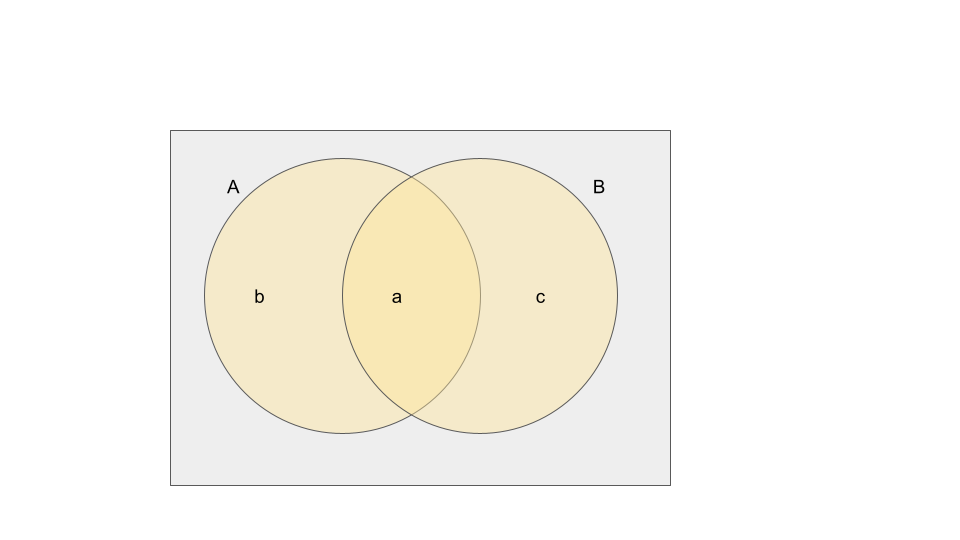
\includegraphics[width=0.7\textwidth]{Theorem_2_7_Venn}
\caption{Theorem 2.7 Venn Diagram}
\label{fig:Venn2.7}
\end{SCfigure}

\newpage
\subsection*{Theorem 2.8 [Discount Triple Check]}
If \(A\), \(B\), and \(C\) are any three events in a sample space \(S\), then
\[
P(A \cup B \cup C) = P(A) + P(B) + P(C) - P(A \cap B) - P(A \cap C) - P(B \cap C) + P(A \cap B \cap C)
\]

\subsubsection*{Proof}
Writing \(A \cup B \cup C \) as \(A \cup (B \cup C) \) and using the formula of Theorem 2.7 twice, once for \(P[A \cup (B \cup C)]\) and once for \(P(B \cup C) \), we get
\begin{align*}
P(A \cup B \cup C) &= P[ A \cup (B \cup C)]\\
&= P(A) + P(B \cup C) - P[A \cap (B \cup C)]\\
&= P(A) + P(B) + P(C) - P(B \cup C) - P[A \cap (B \cup C)]
\end{align*}
Then, using the distributive law that \(A \cap (B \cup C) = (A \cap B) \cup (A \cap C)\):
\begin{align*}
P[A \cap (B \cup C)] &= P[(A \cap B) \cup (A \cap C)] \\
&= P(A \cap B) + P(A \cap C) - P[(A \cap B) \cap (A \cap C)]\\
&= P(A \cap B) + P(A \cap C) - P(A \cap B \cap C)\\
\end{align*}
and hence that
\[
P(A \cup B \cup C)= P(A) + P(B) + P(C) - P(A \cap B) - P(A \cap C) - P(B \cap C) + P(A \cap B \cap C)
\]

\subsection*{Theorem 2.9 [Multiplication Rule]}
If \(A\) and \(B\) are any two events in a sample space \(S\) and \(P(A)\ne 0\), then
\[
P(A \cap B)=P(A) \cdot P(B|A)
\]
Alternatively if \(P(B)\ne 0\), then
\[
P(A \cap B)=P(B) \cdot P(A|B)
\]

\subsection*{Theorem 2.10 [Intersecting 3]}
If \(A, B\), and \(C\) are any three events in a sample space \(S\) such that \(P(A \cap B) \ne 0\), then
\[
P(A \cap B \cap C) = P(A) \cdot P(B|A) \cdot P(C|A \cap B)
\]

\subsubsection*{Proof}
Writing \(A \cap B \cap C\) as \((A \cap B) \cap C\) and using the formula of Theorem 2.9 twice, we get
\begin{align*}
P(A \cap B \cap C) &= P[(A \cap B) \cap C]\\
&= P(A \cap B) \cdot P(C|A \cap B)\\
&= P(A) \cdot P(B|A) \cdot P(C|A \cap B)
\end{align*}


\subsection*{Theorem 2.11 [Independent Complement]}
If \(A\) and \(B\) are independent, then \(A\) and \(B^\complement\) are also independent.

\subsubsection*{Proof}
Since \(A = (A \cap B) \cup (A \cap B^\complement)\), \(A \cap B\) and \(A \cap B^\complement\) are mutually exclusive, and \(A\) and \(B\) are independent by assumption, we have 
\begin{align*}
P(A) &= P[(A \cap B) \cup (A \cap B^\complement)]\\
&= P(A \cap B) + P(A \cap B^\complement)\\
&= P(A) \cdot P(B) + P(A \cap B^\complement)
\end{align*}
It follows that 
\begin{align*}
P(A \cap B^\complement) &= P(A) - P(A) \cdot P(B)\\
&= P(A) \cdot [1 - P(B)]\\
&= P(A) \cdot P(B^\complement)
\end{align*}
and hence that \(A\) and \(B^\complement\) are independent.

\subsection*{Theorem 2.12 [Rule of Total probability or Rule of Elimination]}
If the events \(B_1, B_2, \ldots, B_k\) constitue a partition of the sample space \(S\) and \(P(B_i) \ne 0\) for \(i=1,2,\ldots,k\) then for any event \(A\) in \(S\)
\[
P(A) = \sum_{i=1}^k P(B_i) \cdot P(A|B_i)
\]

\subsection*{Theorem 2.13 [Bayes Theorem]}
If  \(B_1, B_2, \ldots, B_k\) constitute a partition of the sample space \(S\) and \(P(B_i) \ne 0\) for \(i=1,2,\ldots,k\) then for any event \(A\) in \(S\) such that \(P(A) \ne 0\)
\[
P(B_r|A) = \frac{P(B_r) \cdot P(A|B_r)}{\sum_{i=1}^k P(B_i) \cdot P(A|B_i)}
\]
for \(r = 1,2,\ldots,k\)
In words, the probability that event \(A\) was reached via the \(r\)th branch of the following tree diagram, given that it was reached via one of its \(k\) branches, is the ratio of the probability associated with the \(r\)th branch to the sum of the probabilities associated with all \(k\) branches of the tree.

\newpage
\subsubsection*{Proof}
Writing \(P(B_r|A) = \frac{P(A \cap B_r)}{P(A)}\) in accordance with the definition of conditional probability, we have only to substitute \(P(B_r) \cdot P(A|B_r)\) for \(P(A \cap B_r)\) and the formula of Theorem 2.12 for \(P(A)\)
\begin{figure}[h]
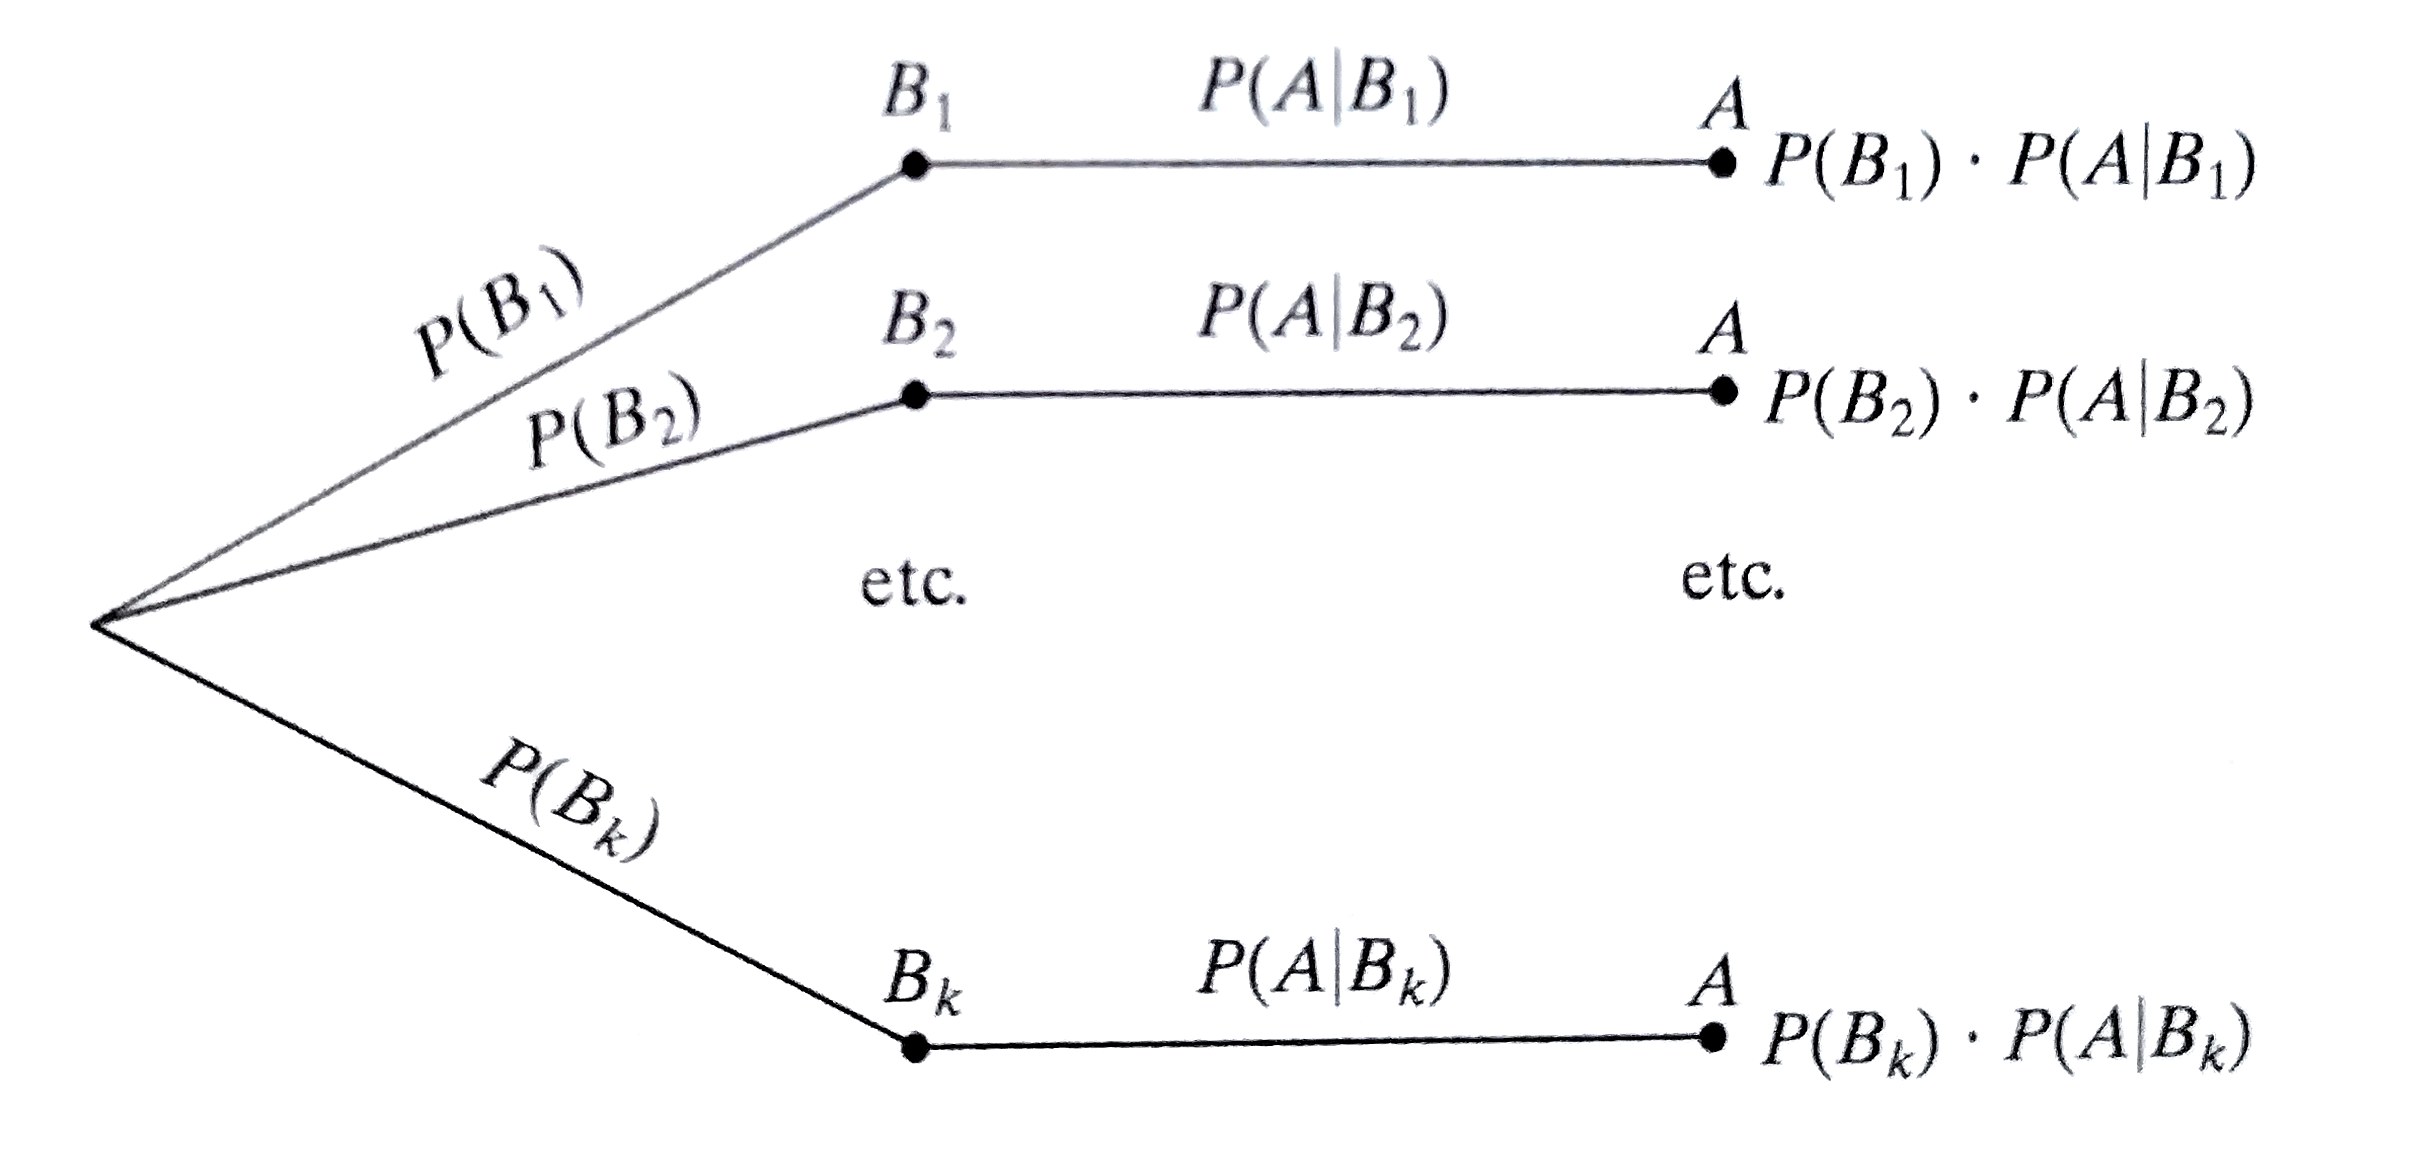
\includegraphics[width=1\textwidth]{BayesTheoremTreeDiagram}
\caption{Bayes Theorem Tree Diagram}
\label{fig:BayesTree}
\end{figure}

\subsection*{Theorem 2.14 [Reliability of a Series System]}
The reliability of a series system consisting of \(n\) independent components is given by 
\[R_s = \prod_{i=1}^n R_i\]
where \(R_i\) is the reliability of the \(i\)th component.

\subsubsection*{Proof}
The proof follows immediately by iterating in Definition 2.5 - Independence

\subsection*{Theorem 2.15 [Reliability of a Parallel System]}
The reliability of a parallel system consisting of \(n\) independent components is given by
\[R_p = 1 - \prod^n_{i=1} (1-R_i)\]

\subsubsection*{Proof}
the proof of this theorem is identical to that of Theorem 2.14, with \((1 - R_i)\) replacing \(R_i\)

\end{document}